\documentclass[12pt]{article}
\usepackage{times}
\usepackage{geometry}
\geometry{letterpaper, portrait, margin=1in}
\usepackage[utf8]{inputenc}
\usepackage{enumitem,amssymb}
\usepackage{ragged2e}
\newlist{thematic}{itemize}{8}
\setlist[thematic]{label=$\square$}
\usepackage{pifont}
\newcommand{\cmark}{\ding{51}}%
\newcommand{\xmark}{\ding{55}}%
\newcommand{\done}{\rlap{$\square$}{\raisebox{2pt}{\large\hspace{1pt}\cmark}}%
\hspace{-2.5pt}}
\newcommand{\wontfix}{\rlap{$\square$}{\large\hspace{1pt}\xmark}}
\usepackage{xcolor}

\begin{document}
\raggedright
\huge
Astro2020 Science White Paper \linebreak

Science Reach with a High-Elevation Radio Instrument, the Beamforming Elevated Array for COsmic Neutrinos \linebreak
\normalsize

\noindent \textbf{Thematic Areas:} \hspace*{60pt} $\square$ Planetary Systems \hspace*{10pt} $\square$ Star and Planet Formation \hspace*{20pt}\linebreak
$\square$ Formation and Evolution of Compact Objects \hspace*{31pt} $\square$ Cosmology and Fundamental Physics \linebreak
  $\square$  Stars and Stellar Evolution \hspace*{1pt} $\square$ Resolved Stellar Populations and their Environments \hspace*{40pt} \linebreak
  $\square$    Galaxy Evolution   \hspace*{45pt} $\checkmark$             Multi-Messenger Astronomy and Astrophysics \hspace*{65pt} \linebreak
  
\textbf{Principal Author:}

Name:	Stephanie Wissel
 \linebreak						
Institution:  California Polytechnic State University
 \linebreak
Email: swissel@calpoly.edu
 \linebreak
Phone:  805-756-7375
 \linebreak
 
\textbf{Co-authors:} (names and institutions)
  \linebreak

\textbf{Abstract  (optional):}


\pagebreak

Call Here:
https://sites.nationalacademies.org/cs/groups/depssite/documents/webpage/deps\_193135.pdf

FAQ Here: 
https://sites.nationalacademies.org/DEPS/Astro2020/DEPS\_192908

10 pages, including figures, but they can be links if necessary

\section{Key Science Goals and Objectives}
\color{blue}
The papers should summarize the most important scientific goals and objectives, justifying the timeliness of the scientific opportunities, and placing them in as broad a context as possible. We encourage the authors, where relevant, to reference Science White Papers submitted to the Survey (these are posted on the Astro2020 website, and may be referenced by author and title). Submitters may also make reference to web sites and other outside materials, but should strive to make this section as self-contained as possible.
\color{black}

High-energy observations of tau neutrinos have the unique capability to address outstanding questions in both astrophysics and fundamental physics, as outlined in three white papers~\cite{Astro2020_fundamental, Astro2020_astrophysics, Astro2020_blazars}. The goals of BEACON, a 100-PeV scale neutrino observatory are:
\begin{enumerate}
	\item Extending the cosmic neutrino spectrum to higher energies	\item Unambiguous detection of an extragalactic source of cosmic neutrinos
 	\item Multi-messenger observations enabled by the highest energy neutrinos at mid-latitudes
	\item Tau fraction can point to different acceleration mechanisms at the sources and possibly beyond-the-standard model physics
\end{enumerate}

%% Make this paragraph sexier
%% This is why we want to extend to higher energies from a multi-messenger 
\textbf{The High Energy End of the Cosmic Neutrino Spectrum} Cosmic neutrino production depends on the assumed acceleration mechanism and source types, both of which are informed by observations by the IceCube neutrino observatory in a lower energy range from 100 TeV to 10 PeV. IceCube has reported on three main analysis of the cosmic neutrino spectrum. Through-going muon neutrinos indicate a hard spectrum with an index of $E^{-2.13\pm0.13}$. Since the neutrino-nucleon cross section grows roughly as $E^{2}$, fully efficient detectors should expect a constant rate of neutrinos across their energy band. However, analyses using the all-flavor and high-energy events contained entirely in the detection tor favor a softer spectral indices of $\sim2.5$. 


The difference in measured spectral indices can be attributed to the energy threshold of the different analyses, meaning that as with photons, the universe mapped in neutrinos is complex. Different sources contribute the neutrino sky and only through improved event statistics, improved angular resolution, extensions to higher energies, and deeper understanding of the flavor composition can we build a complete map of the neutrino sky. 


Active galactic nuclei, pulsars, gamma-ray bursts, and galaxy clusters are all implicated as possible accelerators of ultra-high energy cosmic rays that achieve energies greater than $10^{21}$~eV. The origin of these cosmic rays has confounded the field for decades in part because cosmic rays up to a certain rigidity are unreliable narrators. Such accelerators pump cosmic rays (protons and other nuclei) into the local environment where through $pp$ and $p\gamma$ interactions they can deposit energy into neutrinos, gamma rays, and secondary cosmic rays. Cosmic neutrinos can thus identify the sources of the highest energy particle acceleration in the universe.


Cosmogenic neutrinos are additionally expected at energies above 1 EeV from the interactions of the highest energy cosmic rays with background photons during cosmic ray propagation. Because cosmic rays interact with photon backgrounds within a mean free path of hundreds of megaparsecs and gamma rays are absorbed by the extra galactic background light, cosmogenic neutrinos may provide the only particle probe of the high energy end of the universe at gigaparsec length scales. The long baselines and high energies allow us to probe fundamental physics in otherwise inaccessible energy regimes and length scales~\cite{astro2020_fundamental}.


Two white papers determined the requirements on $>100$ PeV-scale tau neutrino observatories to be \cite{Astro2020_fundamental, Astro2020_astrophysics}:
\begin{itemize}
	\item Energy spectral resolution of half-decade or better to measure cross-sections and spectral features associated with different acceleration mechanisms and BSM physics
	\item High event statistics, of approximately 100 neutrinos of a given flavor
	\item Flavor identification of 40\% or better
	\item Sub-degree pointing resolution
\end{itemize}


With BEACON, we expect to achieve 0.1 degree scale pointing and half-decade energy resolution. Since the number of observed neutrinos is model dependent, and so we expect to either observe as much as 10-30 tau neutrinos over a five year period or place limits on the maximum energy of cosmic ray accelerators and the extension to the diffuse IceCube neutrino flux. 

\section{Technical Overview}
\color{blue}
The team should provide a description of the technical aspects of the pursuit, including a description of the essential performance parameters for achieving the project's science goals.

For ground-based activities/projects, papers should describe the telescope or observatory architecture, key performance requirements, technical requirements, anticipated site and infrastructure requirements, as well as any public/private partnerships.
\color{black}

BEACON targets the sources and flux of tau neutrino by searching for upgoing tau neutrinos that interact within the Earth. Moreover, by using a radio interferometer on a high elevation mountain, the concept maximizes the sensitivity of the instrument at a per channel basis. 
 
\begin{figure}[htbp]
\begin{center}
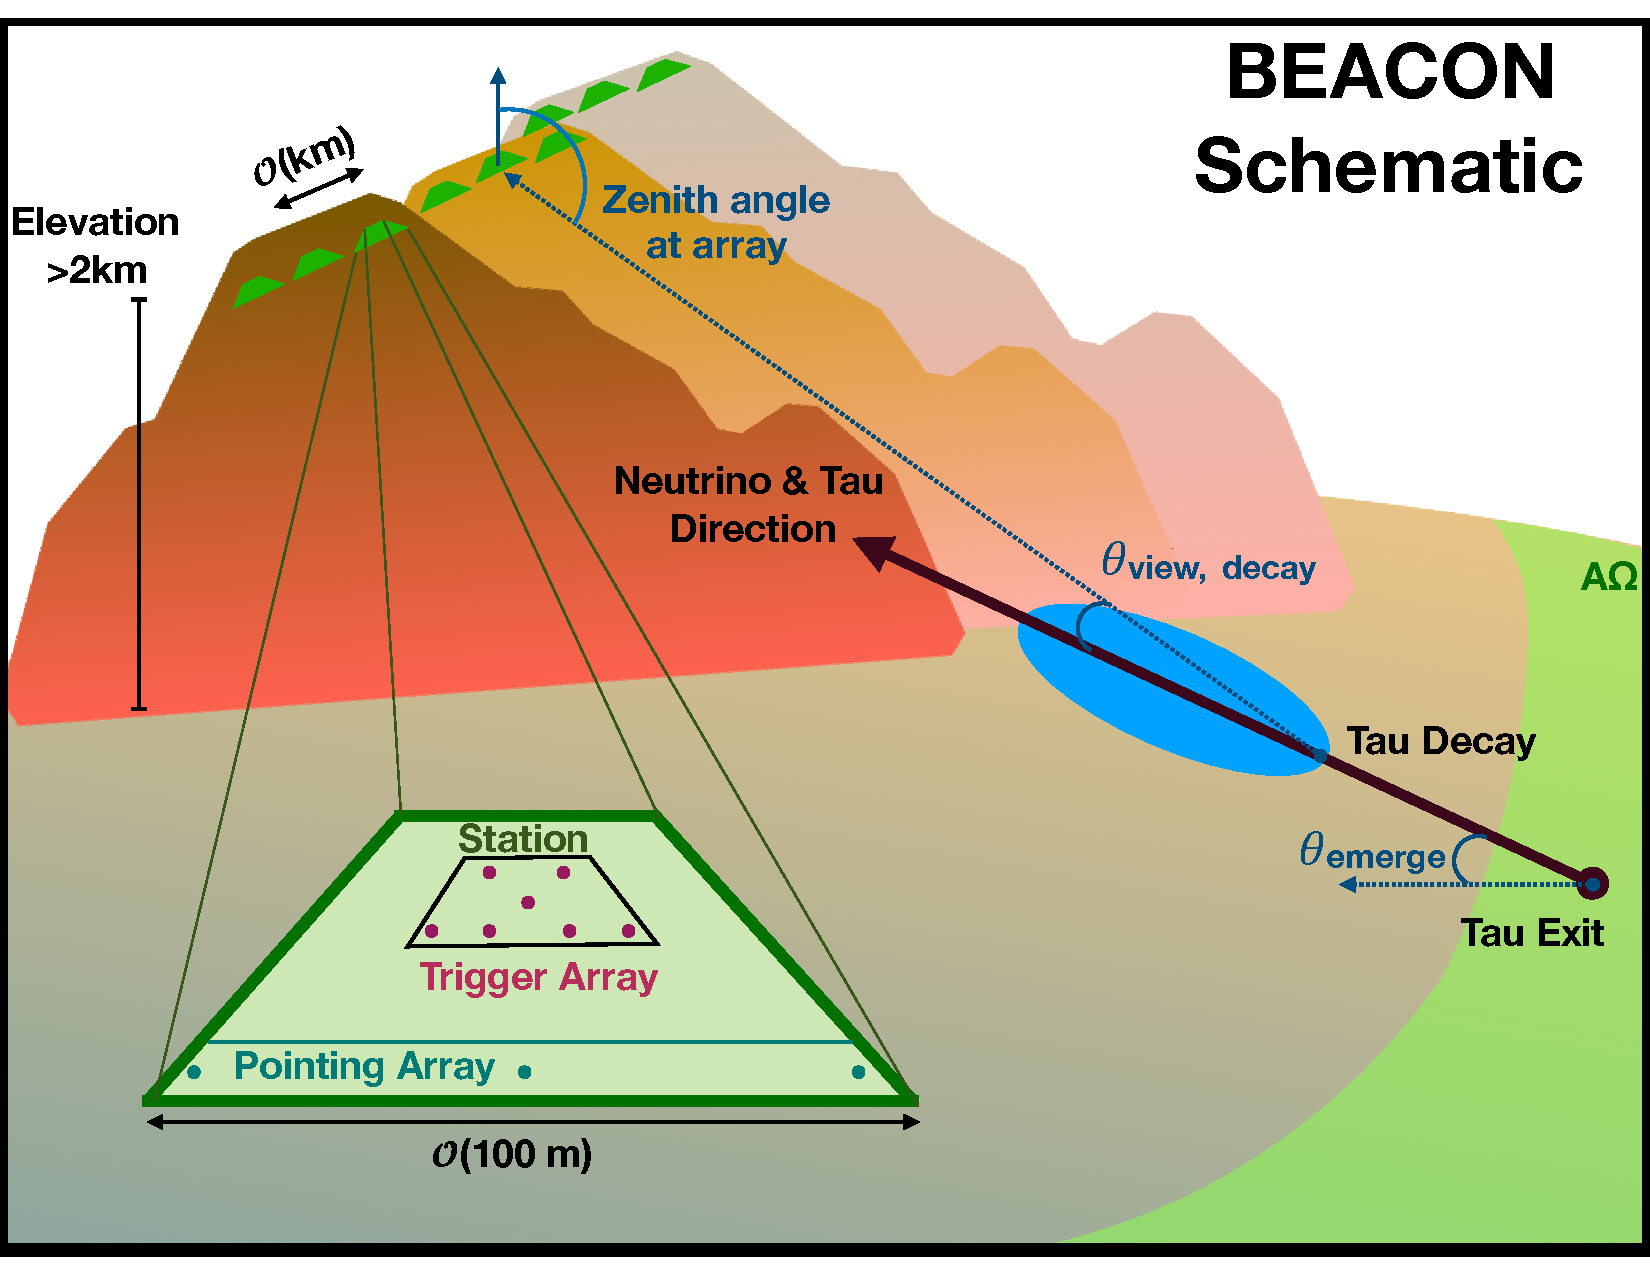
\includegraphics[width=\textwidth]{figures/BEACON_ICRC_Concept.pdf}
\caption{Concept of a high-elevation mountaintop detector.}
\label{fig:concept}
\end{center}
\end{figure}

\begin{figure}[hbtp]
\begin{center}
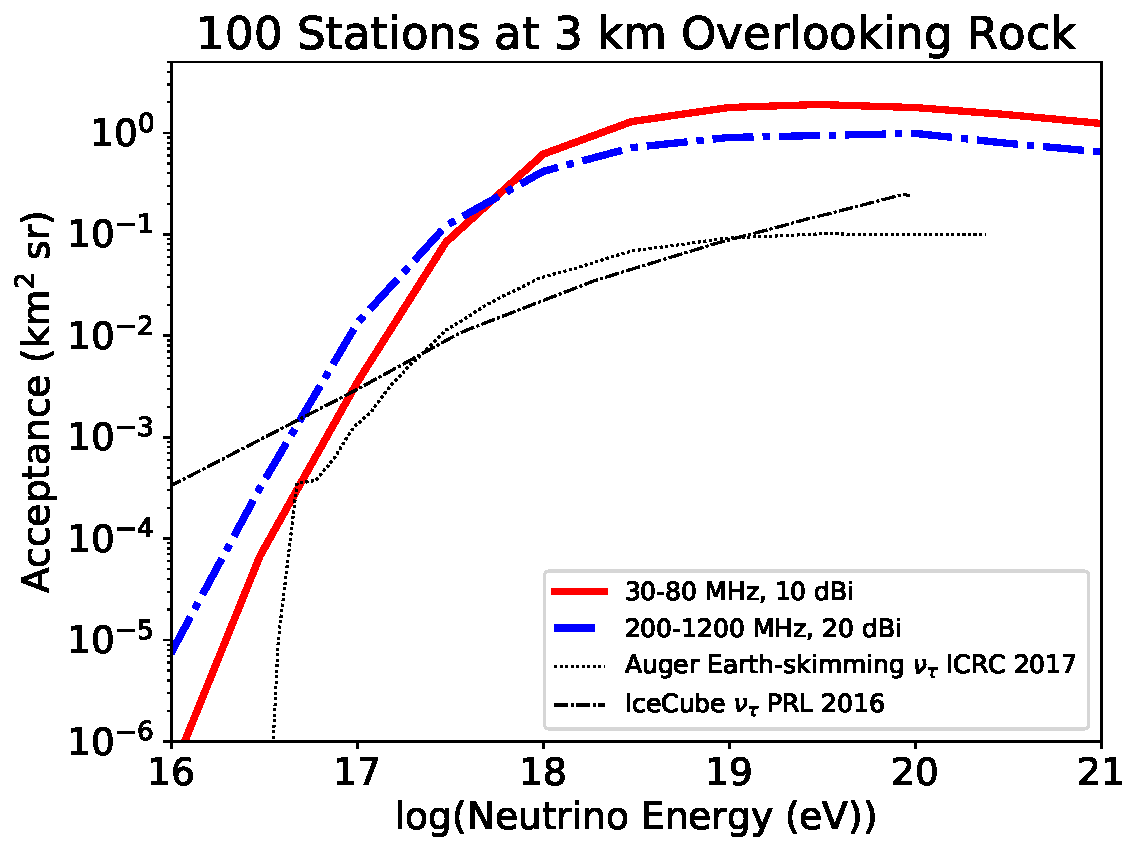
\includegraphics[width=0.54\textwidth]{figures/acceptance_100stations_energyssampling}
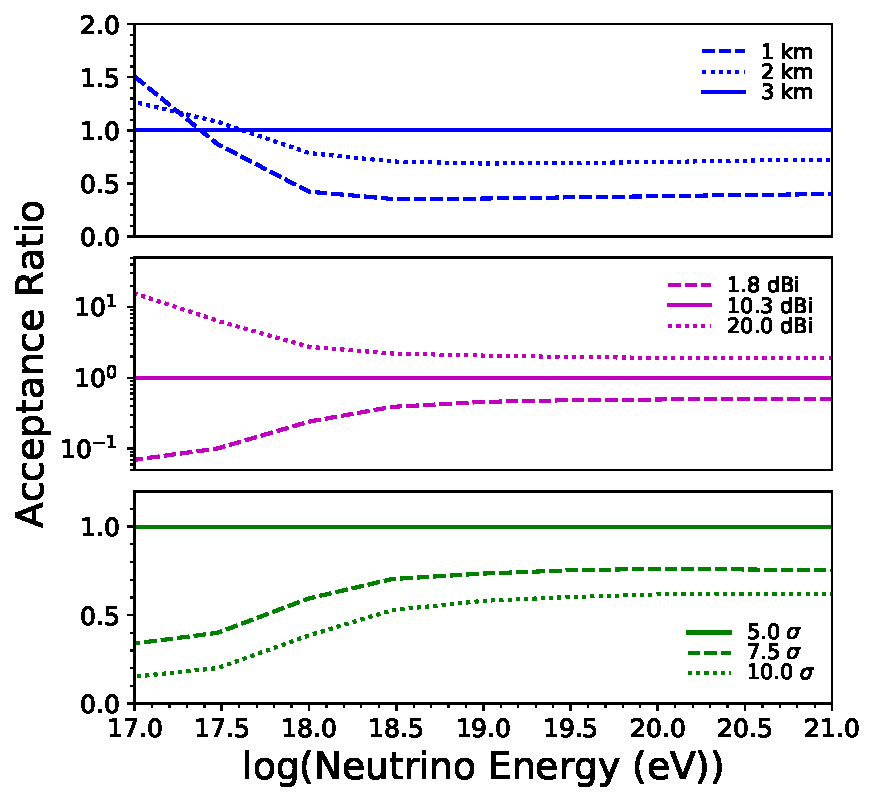
\includegraphics[width=0.45\textwidth]{figures/acceptanceratio_100stations_energyssampling_study}
\caption{(left) The acceptance of BEACON in two different frequency bands compared with the acceptance of PAO to Earth-skimming tau neutrinos and IceCube to tau neutrinos. The designs assume 100 stations at an elevation of 3 km. Each station comprises 7 antennas in the 30-80 MHz range and 10 antennas in the 200-1200 MHz range, both with a threshold of 5$\sigma$. (right) The ratio of the acceptance of a 30-80 MHz detector for different elevations (top), phased array gains (middle), and trigger thresholds (bottom) relative to the reference design. }
\label{fig:acceptance}
\end{center}
\end{figure}

\begin{figure}[tbhp]
\begin{center}
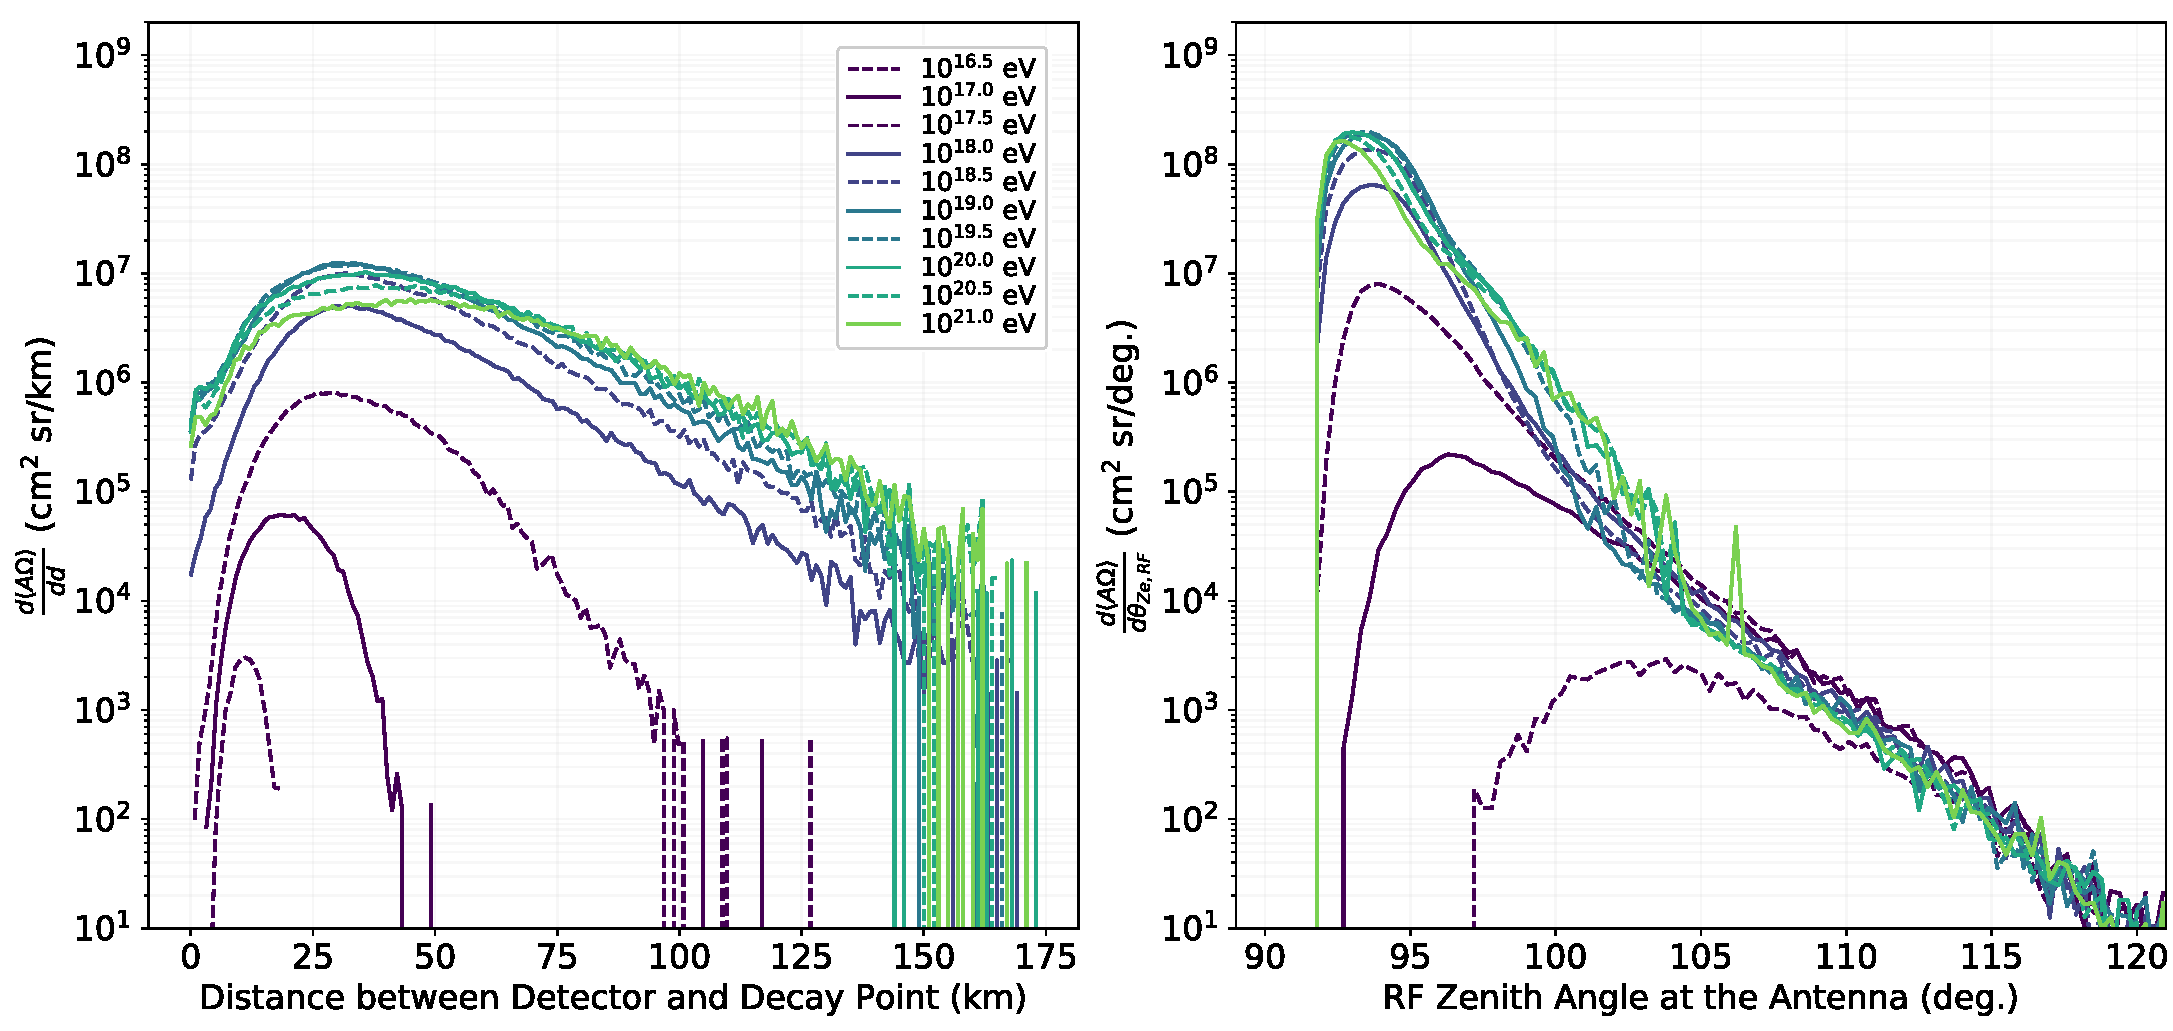
\includegraphics[width=\textwidth]{figures/diffacceptance_30-80MHz_refdesign}
\caption{Differential acceptance of the BEACON reference station to isotropoic tau neutrino flux shows the predominant distances between the decay point and the detector (left) and the zenith angles measured at the array (right) for various energies.}
\label{fig:diffaccep}
\end{center}
\end{figure}

\section{Technology Drivers}
\color{blue}
If the pursuit requires new technologies, the paper should identify and describe them, along with an outline of technology maturation plans and timescales.
\color{black}

\section{Organization, Partnerships, and
Current Status} 
\color{blue}
All pursuits should describe the participating organizations, any planned partnerships, and their current status.
\color{black}

\section{Schedule} 
\color{blue}
The team should outline the development and operations schedule. The schedule should also indicate the operational lifetime of the pursuit.
\color{black}

\section{Cost Estimates}
\color{blue}
 The team should provide any cost estimates that have been developed for the current version of the pursuit. 
 \color{black}

\pagebreak
\textbf{References}



\end{document}

